\documentclass[12pt]{article}

\usepackage{graphicx}
\usepackage[margin=0.75in]{geometry}
\usepackage{multirow}

\begin{document}

\section*{\#3 (a)}

\noindent The density function for the Weibull is 
\[ f(x|\alpha, \lambda) = \alpha\lambda x^{\alpha-1} \exp(-\lambda x^\alpha) \]
with survival function
\[ S(x|\alpha, \lambda) = \exp(-\lambda x^\alpha). \]
\noindent We retain 20,000 posterior samples after a burn-in of 5000. There didn't seem to be any issues regarding convergence.
\bigskip

\noindent I use four different sets of priors:
\begin{enumerate}
\item $p(\alpha)\propto 1/\alpha$, $p(\lambda)\propto 1/\lambda$
\item $\alpha\sim Ga(1, 1)$, $\lambda\sim Ga(1, 1)$
\item $\alpha\sim Ga(1, 1/10)$, $\lambda\sim Ga(1, 1/10)$
\item $\alpha\sim Ga(50, 50)$, $\lambda\sim Ga(50, 50)$
\end{enumerate}
\noindent My preferred set is number 1, since this is non-informative while still not producing an improper posterior. Set 3 is also fairly non-informative, but is a proper prior. Sets 2 and 4 both give priors means to 1 for both parameters, but differ greatly in the prior variance (2 has much larger variance relative to 4).
\bigskip

\noindent From the figures (page 2), only prior set 4 gives much different results than the other 3, which is expected since set 4 is intended to be highly informative.
\bigskip

\noindent The posterior for $\alpha$ is each ploidy group is very similar across all prior sets (note the degree of overlap in the distributions). It may be reasonable to conclude that the value for $\alpha$ is common across the two groups.
\bigskip

\noindent The following table provides a numerical summary for the posteriors in each ploidy group under prior set 1.
\bigskip

\begin{table}[ht]
\centering
\begin{tabular}{ll|rrrr} \hline\hline
Profile & Param & \multicolumn{1}{l}{mean} & \multicolumn{1}{l}{var} &
    \multicolumn{2}{l}{hpd} \\ \hline
\multirow{2}{*}{Aneuploid} & $\alpha$  & 0.827 & 0.015 & 0.584 & 1.066 \\
                           & $\lambda$ & 0.114 & 0.001 & 0.047  & 0.191 \\ \hline
\multirow{2}{*}{Diploid}   & $\alpha$  & 0.774 & 0.018 & 0.513 & 1.050 \\
                           & $\lambda$ & 0.221 & 0.006 & 0.083  & 0.385 \\ \hline\hline
\end{tabular}
\caption{Posterior summaries under prior set 1.}
\end{table}

\begin{center}
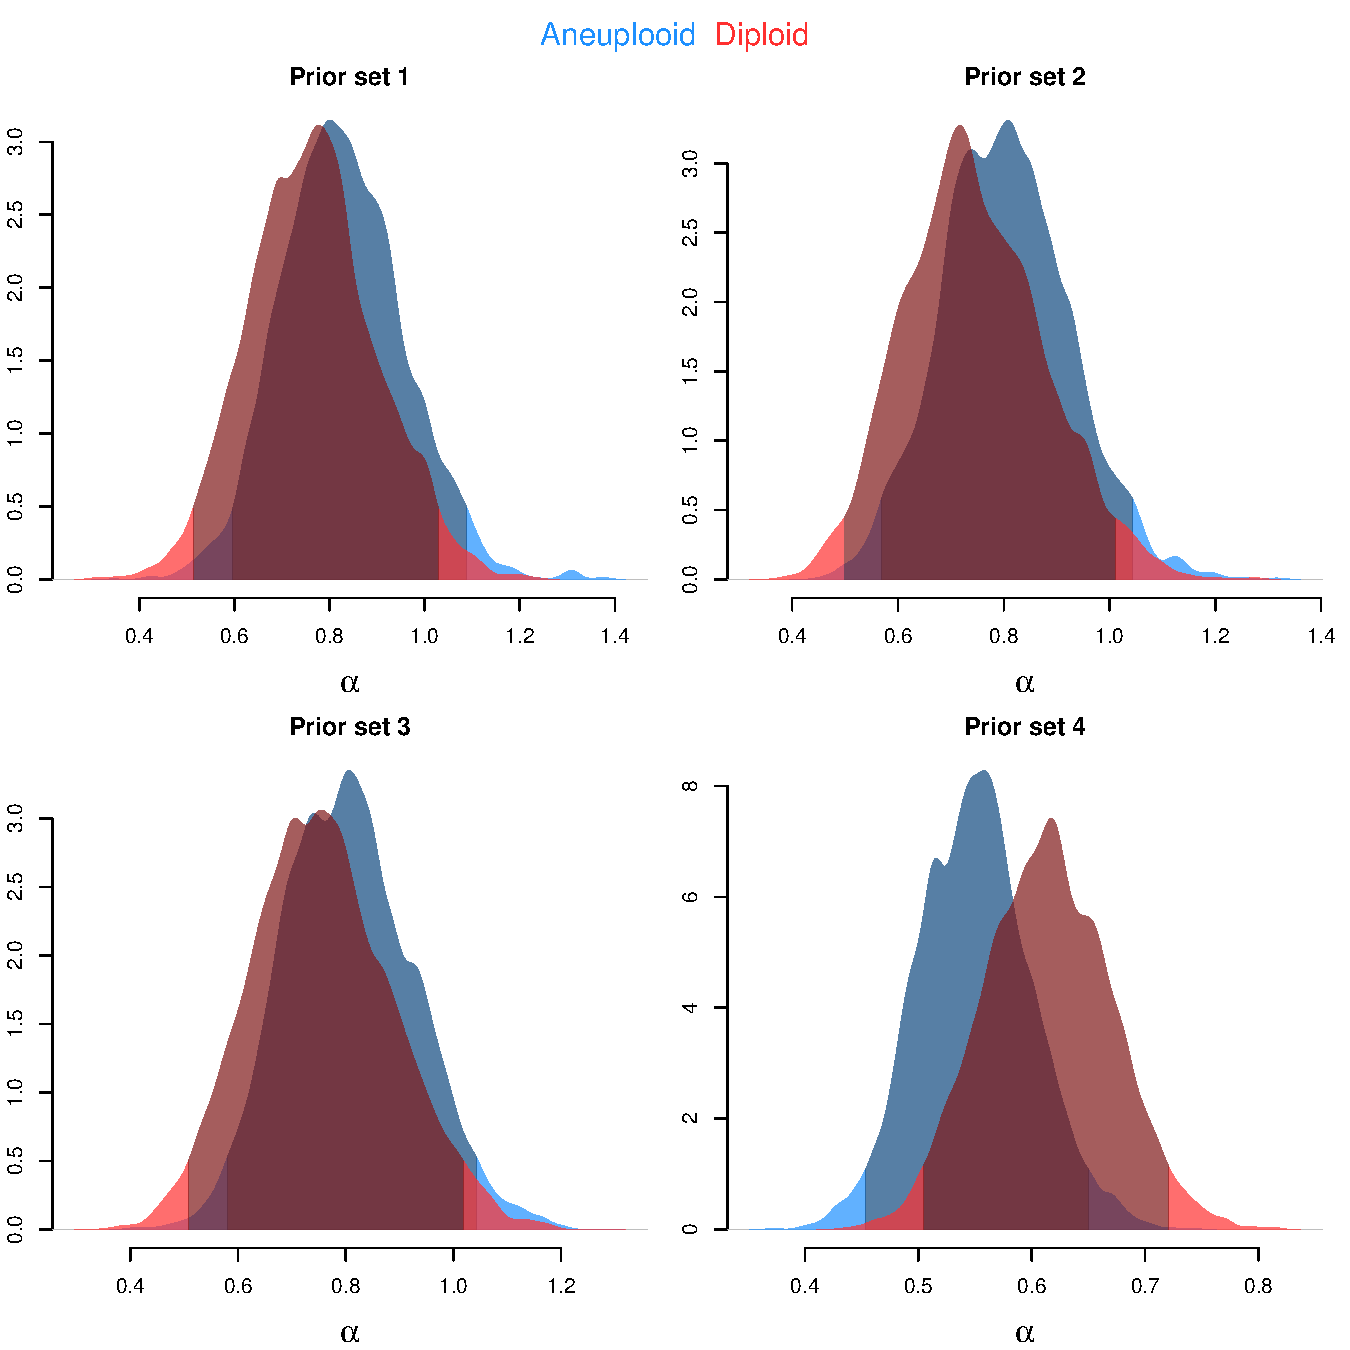
\includegraphics[scale=0.50]{a_sens_alpha.pdf}
\bigskip
\bigskip

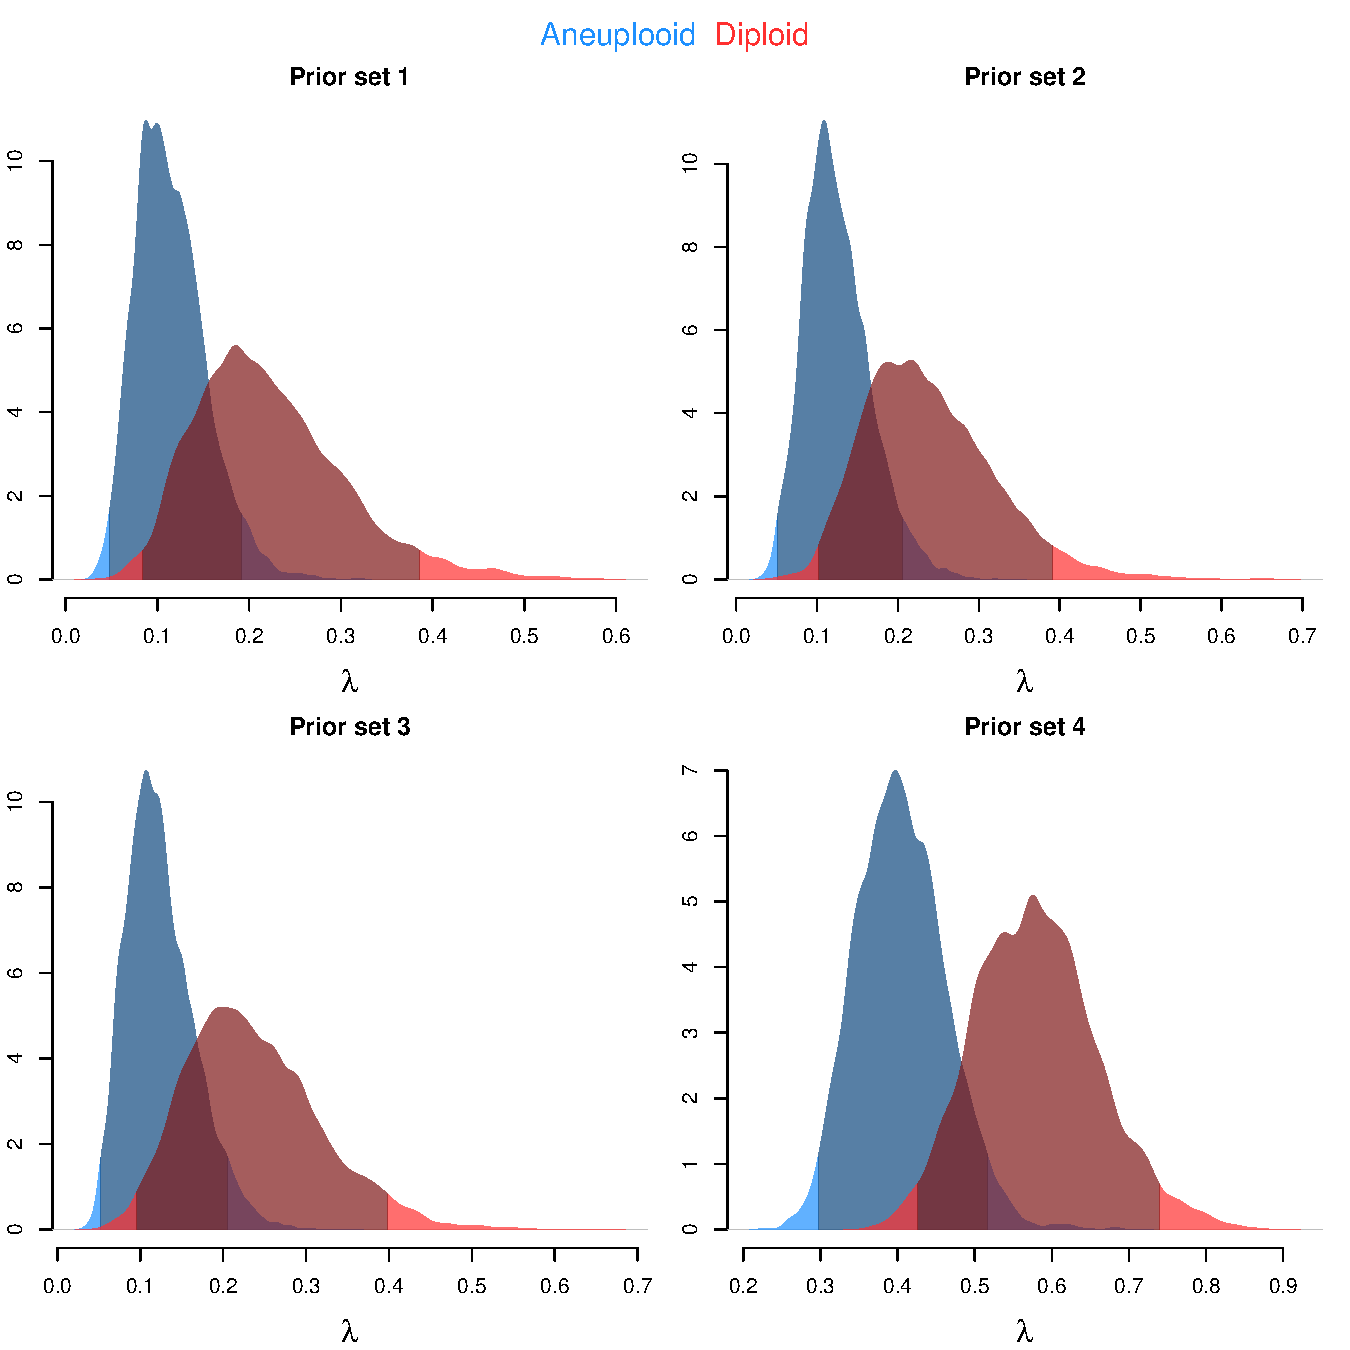
\includegraphics[scale=0.50]{a_sens_lambda.pdf}
\end{center}

\section*{\#3 (b-d)}

\noindent I fit three models to the following:
\[ Y_i = \log T_i = \beta_0 + \beta_1 x_i + \sigma G \]
where $x_i=1$ if the individual is in the aneuploid group and $x_i=0$ if in the diploid group, and $G$ is one of three distributions: extreme value, normal, and logistic (all in standard form). These correspond to having $T$ be distributed either Weibull, log-normal, and log-logistic, respectively.
\bigskip

\noindent The priors for each model are the same:
\[ \beta_0 \sim N(0, 10^2),~~~~~ \beta_1\sim N(0, 10^2), ~~~~~ p(\sigma) \propto 1/\sigma. \]
\noindent These should allow the data to provide a greater contribution to the posteriors. Since I have no expert information to obtain informative priors, I tried to go as non-informative as possible.
\bigskip

\noindent After burning in 5000 samples, we keep 20000 posterior samples to be used in the analysis. There again did not seem to be any issue with convergence.
\bigskip

\noindent The following table provides means, variances, and hpds for the three parameters $(\beta_0, \beta_1, \sigma)$ in each of the three models. Plots of the distributions are shown on the next page. One thing to note as that for each model $\beta_1$ is very similar, whereas for the other parameters, this kind of similarity is not always seen.
\bigskip

\begin{table}[ht]
\centering
\begin{tabular}{ll|rrrrr} \hline\hline
Model & Param & \multicolumn{1}{l}{mean} & \multicolumn{1}{l}{var} &
    \multicolumn{2}{l}{hpd} & \multicolumn{1}{l}{DIC} \\ \hline
\multirow{3}{*}{Weibull}      & $\beta_0$ & 2.022 & 0.078 &  1.484 & 2.589 & \multirow{3}{*}{253.71} \\
                              & $\beta_1$ & 0.689 & 0.141 & -0.091 & 1.423 & \\
                              & $\sigma$  & 1.295 & 0.023 &  1.010 & 1.599 & \\ \hline
\multirow{3}{*}{Log-normal}   & $\beta_0$ & 1.364 & 0.121 &  0.675 & 2.065 & \multirow{3}{*}{253.22} \\
                              & $\beta_1$ & 0.800 & 0.188 & -0.050 & 1.648 & \\
                              & $\sigma$  & 1.748 & 0.032 &  1.399 & 2.093 & \\ \hline
\multirow{3}{*}{Log-logistic} & $\beta_0$ & 1.397 & 0.115 &  0.723 & 2.054 & \multirow{3}{*}{253.45} \\
                              & $\beta_1$ & 0.781 & 0.187 & -0.097 & 1.615 & \\
                              & $\sigma$  & 1.000 & 0.014 &  0.776 & 1.247 & \\ \hline\hline
\end{tabular}
\caption{Posterior summaries for the AFT model.}
\end{table}

\noindent The coefficient $\beta_1$ tells us how to compare the two ploidy groups. Let $T(0)$ be a death time for someone in the diploid group (i.e. $x=0$) and $T(1)$ be the time of death for someone in the aneuploid group ($x=1$). Then we have the following relation with the expected value of the death time
\begin{eqnarray*}
E(T(0)) &=& E(e^{\beta_0+\beta1\times 0+\sigma G}) \\
E(T(1)) &=& E(e^{\beta_0+\beta1\times 1+\sigma G})=e^{\beta_1}\times E(T(0))
\end{eqnarray*}
\noindent For our Weibull model, we estimated $E(e^{\beta_1})\approx2.139$ (note: this is not $e^{0.689}$). This is to say we expect someone in the aneuploid group to live $2.139$ times as long as someone in the diploid group.
\bigskip

\noindent DICs are calculated for each model (shown on the right side of the table). These are all very similar, so selecting which model to use is a matter of taste.

\begin{center}
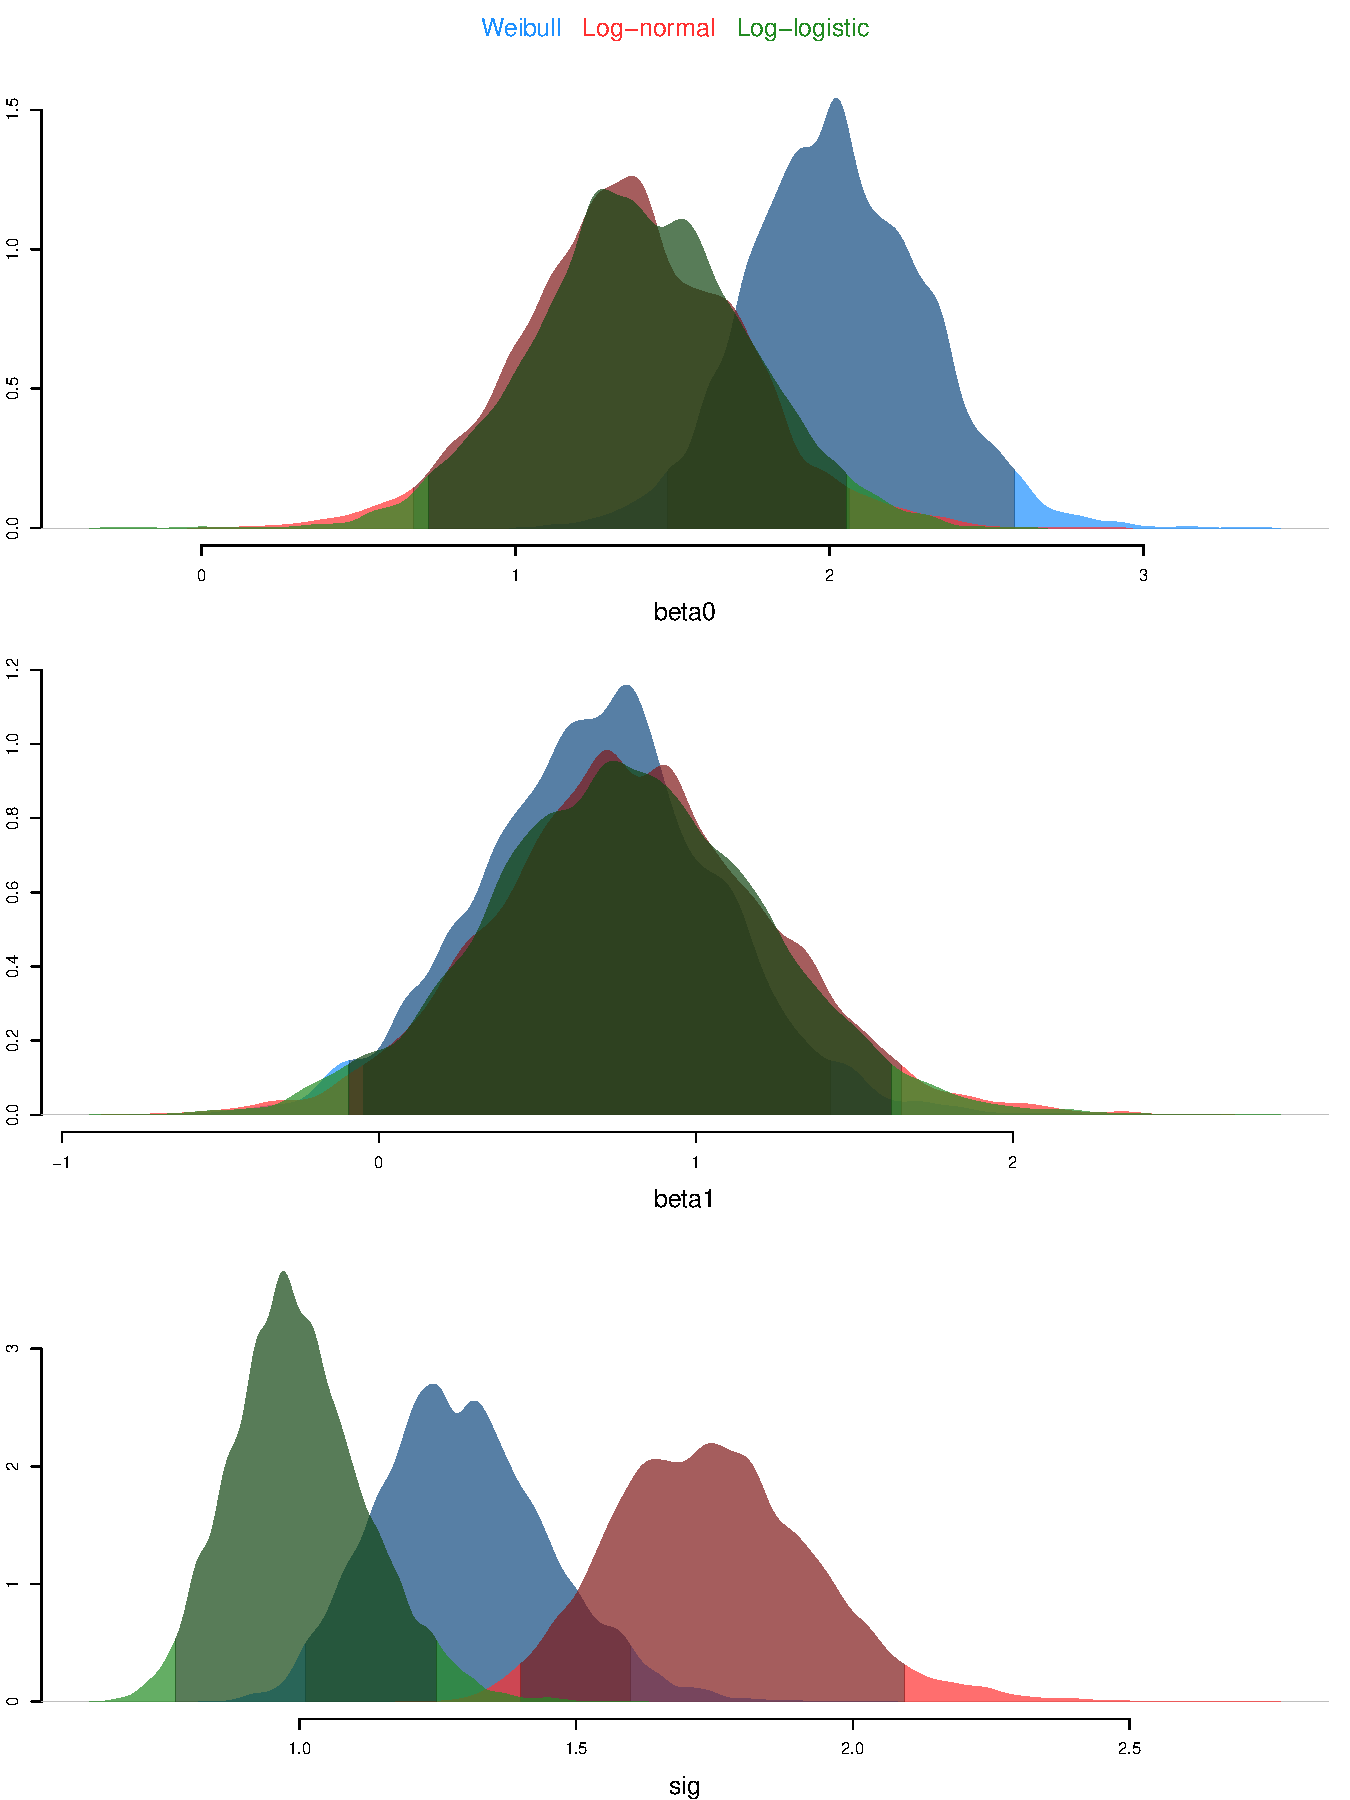
\includegraphics[scale=0.70]{bc_posterior.pdf}
\end{center}


\end{document}
